\begin{tcolorbox}
	\chapter{2013 - Z Mig Na Kuk}
	\paragraph{`Z Miga Na Kuk'} was our first full expedition caving in the longest cave in Slovenia and what better place to begin. 

It was a highly successful 5-weeks of cave exploration on Migovec. Collectively JSPDT and ICCC cavers added another 1.8 km of new cave passage to System Migovec (already the longest cave in Slovenia) bringing the total to an impressive 27.3 km. We were also continuing to camp at `Camp \protect\passage{X-Ray}{}', 600 metres below the surface, and most cavers were spending multiple days underground here. 

We were quite comfortable at this depth and in fact all the findings in \passage{System Migovec} this year were at depths greater than -500m relative to the entrance.

\end{tcolorbox}
	\backgroundsetup{	scale=1,
					color=black,
					opacity=1,
					angle=0,
					contents={%
							  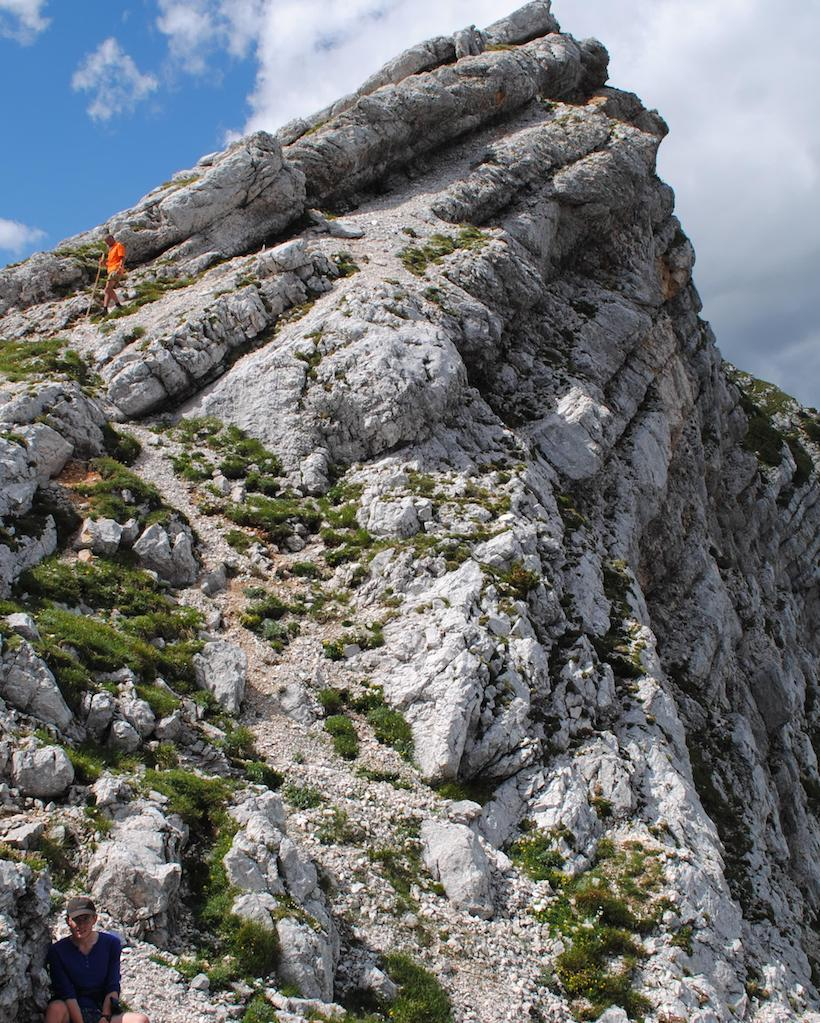
\includegraphics[height=\paperheight]{images/backgrounds/kuk-2013.jpg}
 					 }
	}
\BgThispage
